%!TEX root = *.tex
%%%%%%%%%%%%%%%%%%
% カウンタのリセット
\setcounter{figure}{0}
% 問題文
{
\begin{wrapfigure}{r}{12zw}
  \vspace*{\baselineskip}
  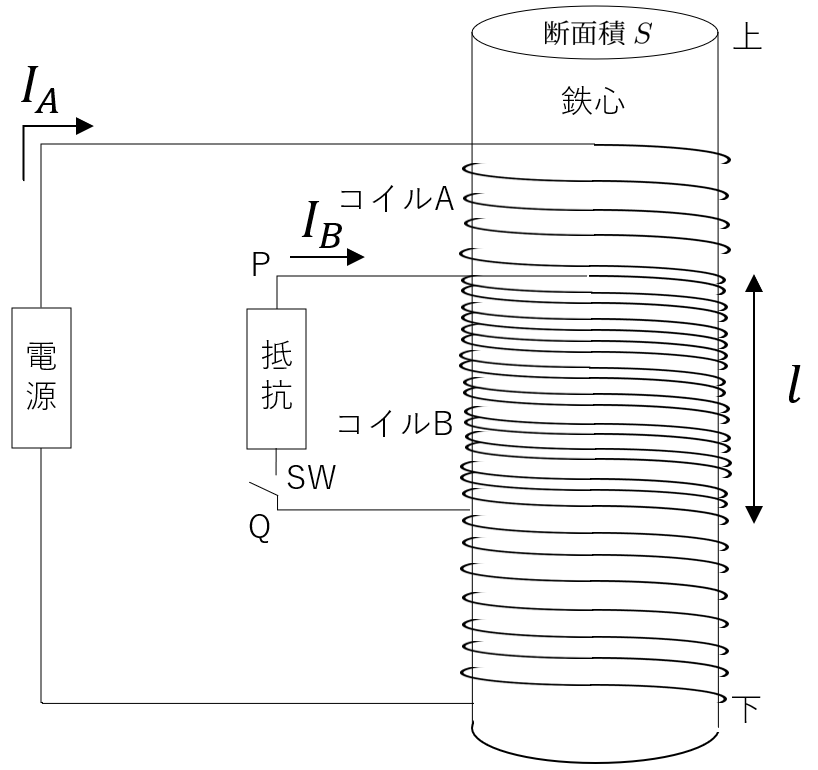
\includegraphics[width=12zw]{../graphs/jumon_132.png}
  \caption{}
\end{wrapfigure}
図1のように,断面積が$S〔\textup{m}^2〕$で透磁率が$\mu〔\textup{N/A}^2〕$の細長い鉄心に,1mあたり\nn 巻きの十分に長いコイルAが巻かれ,その上から長さ$l\unit{m}$で巻き数$N$のコイルBが同じ向きに巻かれて,固定されている.
コイルAには内部抵抗をもつ電源が,コイルBには十分大きな抵抗値$R\unit{Ω}$をもつ抵抗とスイッチSWが,それぞれつながれている.スイッチSWは最初開いている.
コイルAの断面積は,鉄心の断面積$S$に等しく,コイルA内の磁束密度は一様とする.
コイルAを流れる電流により生じた磁束はすべてコイルB内を貫く.
また,導線の抵抗とコイルの抵抗,コイルBに流れる電流による磁束の変化は無視できる.
以下の問い$(1)\sim (5)$に答えよ.

\par}

初めに,コイルAに図1の矢印の向きに$I_A\unit{A}$の電流を流すと鉄心中にコイルAの軸に平行な磁場が生じた.
\begin{enumerate}[(1)]
  \setlength{\leftskip}{-1.5zw}
  \setlength{\itemindent}{1zw}\setlength{\labelsep}{0.5zw}
  \setlength{\labelwidth}{1zw}\setlength{\leftmargin}{1zw}
  \setlength{\itemsep}{0.5\baselineskip}
  \item コイルAの断面を貫く磁束$\Phi\unit{Wb}$を求めよ.また,磁場の向きは上向き,下向きのいずれか答えよ.
\end{enumerate}

次に,微小時間$\Delta t\unit{s}$の間にコイルAの電流を$\Delta I_A\unit{A}$だけ増加させた.
このとき,コイルAを貫く磁束は$\Delta\Phi\unit{Wb}$だけ変化し,コイルBのPとQの間に誘導起電力$V_B\unit{V}$が生じた.
ここで,誘導起電力はQでの値を基準とした.

\begin{enumerate}[(1)]
  \setlength{\leftskip}{-1.5zw}
  \setlength{\itemindent}{1zw}\setlength{\labelsep}{0.5zw}
  \setlength{\labelwidth}{1zw}\setlength{\leftmargin}{1zw}
  \setlength{\itemsep}{0.5\baselineskip}
  \setcounter{enumi}{1}
  \item $V_B$を$\Delta\Phi$を用いて表せ.
  \item $V_B$を$\Delta I_A$を用いて表せ.
  \item このときのAとBの間の相互インダクタンス$M\unit{H}$を求めよ.
\end{enumerate}

今度は,スイッチSWを閉じて,コイルAに流れる電流を$\Delta t$間に$\Delta I_A$だけ増加させた.

\begin{enumerate}[(1)]
  \setlength{\leftskip}{-1.5zw}
  \setlength{\itemindent}{1zw}\setlength{\labelsep}{0.5zw}
  \setlength{\labelwidth}{1zw}\setlength{\leftmargin}{1zw}
  \setlength{\itemsep}{0.5\baselineskip}
  \setcounter{enumi}{4}
  \item このとき,抵抗に流れる誘導電流$I_B\unit{A}$を$\Delta I_A,\,R$を用いて表せ.ただし,電流$I_B$の流れる向きは図1の流れる向きを正とする.
\end{enumerate}




% メモ
\begin{comment}

\end{comment}


%%%%%%%%%%%%%%%%%%
